\chapter{Meditation Requires Order}

We begin with a warning about meditation. In this talk, meditation is not introduced as a practice, a posture, a ten-minute exercise, or a private technique for producing calm. Krishnamurti asks what kind of mind is capable of meditation at all. The answer is not given immediately. The lecture proceeds by clearing the ground: freedom, violence, choice, time, disorder, love, and death must all be understood before meditation can be anything other than escape.

The chapter will use a small amount of symbolic notation. None of it is blackboard notation from the lecture. There were no validated board images for this talk. The symbols are only compact scaffolding for the argument, useful in the same way a diagram is useful: they show the structure of the inquiry without replacing the spoken movement.

\section{Meditation Begins With Freedom}

The first question is not, ``How does one meditate?'' The first question is: what is necessary for a mind that is capable of true meditation? Krishnamurti's answer begins with freedom.

But freedom is immediately split into two meanings. There is outward freedom: political freedom, freedom of expression, freedom to think what one likes, freedom to choose, freedom from a particular habit. And there is inward freedom: freedom from the mind's own projections, demands, desires, fulfillments, cravings, and appetites.

We can write the first distinction schematically as
\begin{equation}
F_{\mathrm{out}} \not\Rightarrow F_{\mathrm{in}} .
\end{equation}
This is not a formal theorem. It is a way of remembering the first movement of the lecture: outward freedom, though necessary in its own field, does not by itself make the mind free.

\begin{definition}
Let \(F_{\mathrm{out}}\) denote outward freedom: political, social, expressive, and choice-based freedom. Let \(F_{\mathrm{in}}\) denote inward freedom: freedom from projection, craving, appetite, violence, fear, dependence, authority, and conditioning.
\end{definition}

The lecture grants political freedom its importance. One must have it. But then it asks why we rarely inquire into inward freedom. The mind may be outwardly permitted to choose and still be inwardly enslaved to its own movement.

That is why meditation cannot begin as a method. If the mind is not free, method only gives the unfree mind another pattern to follow.

\section{Choice, Violence, And The Verb To Be}

The next step is deliberately unsettling. We commonly equate freedom with choice. Krishnamurti reverses that assumption. Where there is clear seeing, he says, there is no choice; there is only action. Choice belongs to confusion, not clarity.

The early argument may be compressed as
\begin{align}
\mathrm{Clarity} &\Rightarrow \mathrm{No\ Choice} \Rightarrow \mathrm{Action}, \\
\mathrm{Choice} &\Rightarrow \mathrm{Confusion} \Rightarrow \mathrm{Resistance/Conflict}.
\end{align}
This is a useful map of the spoken argument. It should not be read as a mechanical law. The point is sharper than that: choice, in the psychological field, is not a sign of freedom if it arises because the mind does not see clearly.

\subsection{Question \& Answer}

\paragraph{Question.}
If choice is usually taken to be freedom, why does the lecture say that choice indicates a lack of freedom?

\paragraph{Answer.}
Because the lecture is not speaking about practical selection among ordinary alternatives. It is examining the mind that chooses because it is divided, uncertain, and confused. When a thing is seen clearly, there is no inner bargaining between alternatives. The seeing itself is action. A confused mind chooses, resists, compares, and enters conflict; therefore choice in this sense belongs to disorder rather than freedom.

From choice the lecture moves to violence. Violence is not restricted to war or physical aggression. It includes the inward structure of resistance and conflict. A society that insists on outward change without inward change still carries violence at its centre.

We may summarize the relation cautiously:
\begin{equation}
\mathrm{Violence} \supset
\{\mathrm{choice},\ \mathrm{conflict},\ \mathrm{outward\ change\ without\ inward\ change}\}.
\end{equation}
The notation is only editorial. It marks that violence, for the purposes of this lecture, has a much wider field than obvious aggression.

Then Krishnamurti names a deeper conditioning: the verb ``to be.'' The mind is organized by becoming:
\begin{equation}
\mathrm{To\ Be}:\qquad
\mathrm{has\ been} \longrightarrow \mathrm{is} \longrightarrow \mathrm{will\ be}.
\end{equation}
In that verb lie arrival, success, achievement, becoming, gradual attainment, and gradual removal of obstacles. The moral structure of the mind is built around it: I will be good; I will gradually achieve a certain state.

This is the conditioning of the mind in time.

\section{Time As Becoming}

The critique of psychological time is the hinge of the lecture. It connects choice and violence with false spirituality. If the mind says, ``I will gradually become peaceful,'' it has already accepted the structure of becoming. It has placed freedom, order, love, or enlightenment in the future.

The lecture's counterclaim is direct:
\begin{equation}
\mathrm{Understanding} \neq
\lim_{t\to\infty}\mathrm{Gradual\ Improvement}(t).
\end{equation}
This equation is intentionally schematic. It does not appear in the talk. It gives mathematical shape to a verbal insistence: understanding is not a matter of gradual sensitivity. Either one understands immediately, or one does not understand.

\begin{remark}
The word ``immediately'' here should not be made into a doctrine of sudden achievement. The point is negative: understanding is not produced by the time-structure of becoming. It is not the end point of a psychological accumulation.
\end{remark}

The danger of the word is therefore part of the danger of time. The word is not the thing; the description is not the described. Yet the mind is satisfied with descriptions, explanations, and promises of future arrival.

At this point the lecture returns to meditation only to postpone it again. Before meditation can be understood, one must understand living, love, and death. Otherwise meditation is merely an escape, a form of self-hypnosis.

\section{Living As Disorder}

The foundation for meditation is not an idea of order but the observation of actual living. The lecture now turns from the abstract structure of becoming to the concrete disorder of daily life.

Actual life is described as conflict, driving ambition, battle within oneself, contradictory desires and wills, frustration, comparison, escape, loneliness, routine, division, and self-centred activity. The centre that demands fulfillment is itself questioned: is not that very centre the cause of disorder?

The basic opposition can be written as
\begin{equation}
\mathrm{What\ Is} \neq \mathrm{What\ Should\ Be}.
\end{equation}
When the mind lives between these two poles, there is conflict:
\begin{equation}
\mathrm{Conflict}(\mathrm{What\ Is},\mathrm{What\ Should\ Be})
\Rightarrow
\mathrm{Disorder}.
\end{equation}

This is the lecture's first worked example of disorder.

\begin{proof}
Consider the mind that observes its actual state: ambition, fear, envy, loneliness, or frustration. If it immediately compares that state with an ideal state, what should be, it has introduced a second image. The actual fact and the projected image now oppose one another. That opposition is conflict. Since this conflict is the ordinary movement of daily life, the life itself is disorder.
\end{proof}

The phrase ``complete mathematical order'' appears here, but it should be handled carefully. It does not introduce a calculus or a formal system. It points to completeness: order cannot be partial, imposed, or merely outward. Without order in the actual life one lives, meditation has no foundation.

The lecture then asks the question that the whole description has prepared.

\subsection{Question \& Answer}

\paragraph{Question.}
How can that life, the life of conflict, comparison, escape, and fear, be changed?

\paragraph{Answer.}
Not gradually. If change is postponed into gradual becoming, the same structure of violence continues. The change begins with seeing the fact non-verbally, not as explanation or idea, but as something as direct as hunger. One must be intimately related to what is, without escape and without distortion.

\section{Observation, Discipline, And Order}

The central relation of the lecture is now visible. Order is not imposed upon disorder. Order comes from observing disorder without choice and without distortion.

We can write the movement as
\begin{align}
\mathrm{Observation}_{\mathrm{no\ choice,\ no\ distortion}}(\mathrm{Disorder})
&\Rightarrow \mathrm{Learning}, \\
\mathrm{Learning} &\Rightarrow \mathrm{Discipline}, \\
\mathrm{Discipline} &\Rightarrow \mathrm{Order}.
\end{align}

The word discipline is important. It does not mean conformity, imitation, suppression, or obedience to an imposed pattern. It means learning. In the very act of observing, one learns, and that learning has its own discipline.

\begin{figure}
\centering
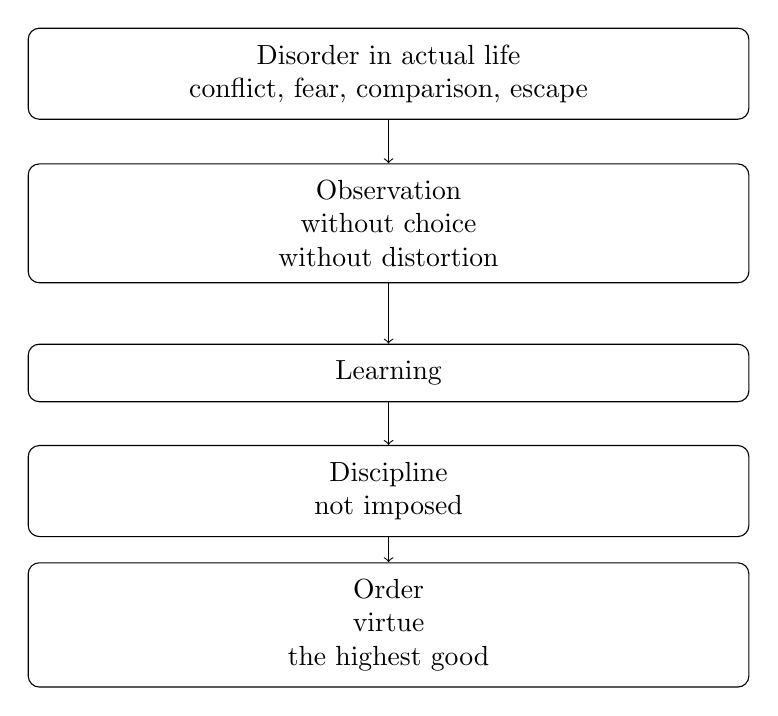
\begin{tikzpicture}[
  node distance=1.0cm,
  box/.style={draw, rounded corners, align=center, text width=0.72\linewidth, inner sep=6pt}
]
\node[box] (d) at (0,0) {Disorder in actual life\\conflict, fear, comparison, escape};
\node[box] (o) at (0,-1.9) {Observation\\without choice\\without distortion};
\node[box] (l) at (0,-3.8) {Learning};
\node[box] (disc) at (0,-5.3) {Discipline\\not imposed};
\node[box] (ord) at (0,-7.0) {Order\\virtue\\the highest good};
\draw[->] (d) -- (o);
\draw[->] (o) -- (l);
\draw[->] (l) -- (disc);
\draw[->] (disc) -- (ord);
\end{tikzpicture}
\caption{A transcript-backed reconstruction of the lecture's movement from observed disorder to order. No screenshot is available for this diagram.}
\end{figure}

The crucial step is that we do not move from disorder to an idea of order. If we impose what we think order should be upon disorder, we create another conflict between what is and what should be. That is still disorder.

The lecture then turns outward for contrast. Every outward revolution that tries to make state order first, while forgetting inward order, repeats the same error. Outward order without inward order has never solved the problem.

\begin{equation}
\mathrm{Inward\ Order} \Rightarrow \mathrm{Outward\ Order},
\qquad
\mathrm{Outward\ Order} \not\Rightarrow \mathrm{Inward\ Order}.
\end{equation}

This is the political and psychological pivot of the talk. The order required for meditation is not state order, social discipline, or imposed morality. It is the order that arises when disorder is seen without distortion.

\section{Love Through Negation}

Order is then linked to virtue and love. The transition is not ornamental. If order is the ending of conflict, and if conflict is bound up with fear, comparison, and self-centred movement, then love cannot be understood apart from order.

Krishnamurti asks: what is love? The answer is approached through negation. One finds out what it is by seeing what it is not.

\begin{equation}
\mathrm{Love} \notin
\{\mathrm{jealousy},\mathrm{envy},\mathrm{comparison},\mathrm{pleasure},
\mathrm{dependence},\mathrm{fear},\mathrm{authority},\mathrm{conditioning}\}.
\end{equation}

Again, the notation is not a definition of love. It is a map of the exclusions by which the lecture proceeds.

\subsection{Question \& Answer}

\paragraph{Question.}
Can love be cultivated?

\paragraph{Answer.}
No. Cultivation belongs to thought and becoming. A proud mind that cultivates humility remains proud in its very cultivation. In the same way, a mind that sets out to cultivate love is still operating through projection, time, and the desire to become. Therefore the lecture asks us to see what love is not, and to let the false disappear in the seeing.

The first negations are jealousy and envy. Love hedged about by jealousy is not love. Envy arises with comparison, and the lecture asks directly whether love can be comparison. If comparison ends, envy loses its ground.

The more difficult negation is pleasure. Pleasure is sustained by thought. A remembered experience is carried over, thought builds image upon image, the image stimulates, and that stimulation is called pleasure. The talk compresses this process:
\begin{equation}
\mathrm{Remembered\ Pleasure}
\xrightarrow{\ \mathrm{thought}\ }
\mathrm{Image\ upon\ image}
\xrightarrow{\ \mathrm{stimulation}\ }
\mathrm{Pleasure}.
\end{equation}

The problem is not enjoyment as such. The problem is the psychological machinery that turns memory, image, and dependency into what we call love. In pleasure there is frustration, pain, agony, and dependence. And in dependence there is fear.

\begin{align}
\mathrm{Dependence} &\Rightarrow \mathrm{Fear}, \\
\mathrm{Pleasure\ as\ image} &\Rightarrow \mathrm{Dependence}, \\
\therefore\quad \mathrm{Pleasure\ as\ image} &\Rightarrow \mathrm{Fear}.
\end{align}

This is a worked logical chain, not a clinical theory. It preserves the lecture's sequence: thought sustains pleasure, pleasure carries dependence, dependence contains fear, and what contains fear cannot be love.

The lecture then widens the inquiry. We are conditioned by society, propaganda, education, books, authority, and memory. Experience itself is old if it is recognized, because recognition is the response of memory. Thought is old for the same reason. Thus the human being becomes second-hand: intellectually, emotionally, morally.

Love cannot be second-hand.

\section{Death And The Ending Of The Known}

To understand love, the lecture says, one must also understand death. This is not a new topic placed beside the others. Living, love, and death are to be seen as one movement:
\begin{equation}
\mathrm{Life} \neq
\{\mathrm{Living}\}\cup\{\mathrm{Love}\}\cup\{\mathrm{Death}\}
\quad\hbox{as separate compartments.}
\end{equation}
A cleaner way to say it in prose is: life includes living, love, and death as a total movement.

Krishnamurti first acknowledges biological death. The organism comes to an end through age, disease, usage, accident, and conflict. But he does not remain with biological ending. He asks about the ending of the ``me,'' the centre that divides itself as us and they, we and you, and therefore becomes the centre of conflict.

\subsection{Question \& Answer}

\paragraph{Question.}
Can the ``me'' die, not eventually, but every day?

\paragraph{Answer.}
That is the lecture's practical question about death. To die every day is to end one's psychological accumulation: pleasure, knowledge, memory, and the furniture of the mind. It is not an idea about afterlife. It is the ending of the known in the present.

We can summarize the distinction:
\begin{align}
\mathrm{Death}_{\mathrm{bio}} &=
\mathrm{Ending\ of\ the\ organism}, \\
\mathrm{Death}_{\mathrm{psych}} &=
\mathrm{Ending}(\mathrm{me},\mathrm{known},\mathrm{pleasure},\mathrm{accumulation}).
\end{align}

The lecture does not ask us to believe in reincarnation or disbelieve in it. Even if one believes in reincarnation, it says, what matters is how one lives now. The point is always brought back to present living.

The final movement is stark:
\begin{equation}
\mathrm{Ending\ the\ Known} \Rightarrow \mathrm{Innocence\ of\ Mind}.
\end{equation}
Only such a mind, emptied of the known, can come upon what Krishnamurti calls enlightenment. The wording matters: it can come upon it. Enlightenment is not presented as an achieved object, a result of time, or a prize of method.

\section{Summary}

The lecture begins with meditation and then refuses every shortcut to meditation. First comes freedom, but freedom is not choice. Choice belongs to confusion; clarity acts. Then comes violence, not merely as outward aggression but as the inward movement of conflict, resistance, and outward change without inward transformation.

The deeper structure is the verb ``to be,'' the mind's movement through psychological time: has been, is, will be. As long as the mind is organized by becoming, it turns even morality, order, love, and enlightenment into future achievements.

The foundation for meditation is therefore the understanding of actual living. Actual living is disorder when it is governed by conflict, comparison, escape, ambition, fear, and the division between what is and what should be. The change in such a life is not gradual. It comes through observing disorder without choice and without distortion. That observation is learning; learning is discipline; discipline is order.

Order then opens into love, and love is approached through negation. It is not jealousy, envy, comparison, pleasure, dependence, fear, authority, or second-hand conditioning. Finally, love cannot be separated from death. Death is not only the ending of the organism but the daily ending of the ``me,'' the known, pleasure, and accumulation. In that ending, the mind becomes innocent, and only such a mind is capable of true meditation.